% Archive record 58, line 7.
\hypertarget{part-4-58-0007-iv-a-ux6ce2ux52a8ux7387ux805aux96c6ux539aux5c3eux4e0eux65f6ux95f4ux4f9dux8d56}{%
\section{IV-A --- 波动率聚集、厚尾与时间依赖}\label{part-4-58-0007-iv-a-ux6ce2ux52a8ux7387ux805aux96c6ux539aux5c3eux4e0eux65f6ux95f4ux4f9dux8d56}}

\hypertarget{part-4-58-0007-volatility-clusteringux6ce2ux52a8ux7387ux805aux96c6}{%
\subsubsection{6.2 Volatility Clustering（波动率聚集）}\label{part-4-58-0007-volatility-clusteringux6ce2ux52a8ux7387ux805aux96c6}}

金融市场中的高波动通常倾向于连续出现，低波动时期也可能持续一段时间。

\begin{readerfigure}{0.87}
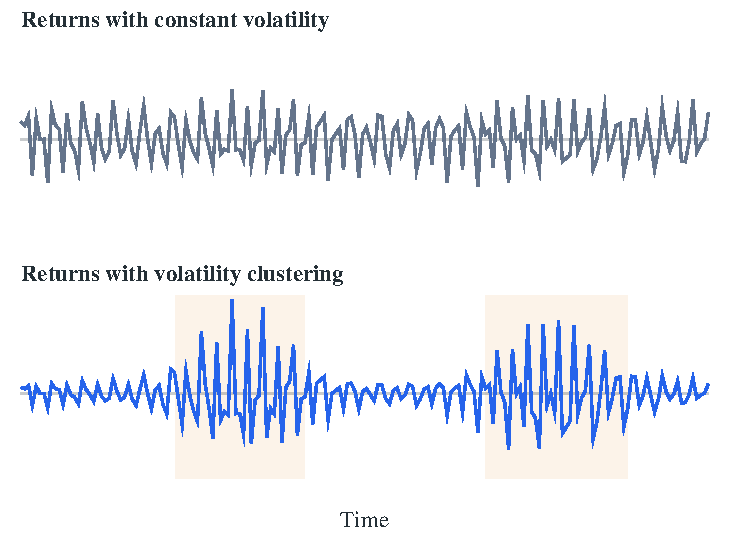
\includegraphics[width=\linewidth]{../reader_prototype/latex/figures/volatility.pdf}
\captionof{figure}{合成示意：右侧序列的收益率方向难以预测，但波动幅度具有明显的持续性。}
\end{readerfigure}

因此，在金融数据中，我们可能同时观察到：
\[\operatorname{Corr}(r_t,r_{t+h})\approx0,\]

但：
\[\operatorname{Corr}(|r_t|,|r_{t+h}|)>0,\]

或者：
\[\operatorname{Corr}(r_t^2,r_{t+h}^2)>0.\]

这意味着：

\textbf{收益率本身可能不具有明显的线性可预测性，但其波动程度具有可预测性。}

\begin{readerfigure}{0.87}
\figuretitle{Typical Financial Return ACF}
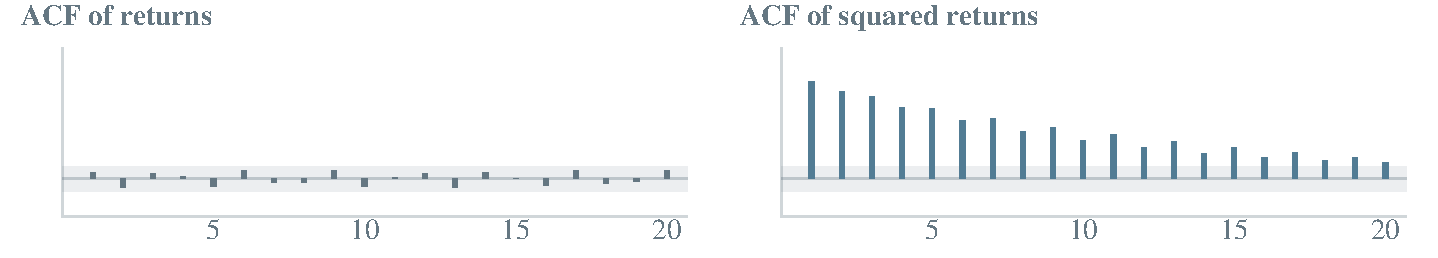
\includegraphics[width=\linewidth]{../reader_prototype/latex/figures/acf.pdf}
\captionof{figure}{典型形态的教学示意，非实际市场数据。原始收益率的自相关接近零，平方收益率的自相关则可能缓慢衰减。}
\end{readerfigure}

\hypertarget{part-4-58-0007-ux4e00ux4e2aux4e25ux683cux7684ux6982ux7387ux53cdux4f8b}{%
\subsubsection{6.3 一个严格的概率反例}\label{part-4-58-0007-ux4e00ux4e2aux4e25ux683cux7684ux6982ux7387ux53cdux4f8b}}

为了进一步理解为什么 Uncorrelated 不等于 Independent，我们构造一个非常简单的随机过程。 设：
\[Z_t\overset{\mathrm{i.i.d.}}{\sim}\mathcal N(0,1),\]

并定义：
\[r_t=Z_tZ_{t-1}.\]

首先，由独立性：
\[\mathbb E[r_t]
=
\mathbb E[Z_t]\mathbb E[Z_{t-1}]
=0.\]

\hypertarget{part-4-58-0007-proposition-1-returns-are-uncorrelated}{%
\paragraph{Proposition 1 --- Returns are uncorrelated}\label{part-4-58-0007-proposition-1-returns-are-uncorrelated}}

相邻收益率的协方差为：
\[\begin{aligned}
\operatorname{Cov}(r_t,r_{t+1})
&=\mathbb E[r_tr_{t+1}]\\
&=\mathbb E[Z_t^2Z_{t-1}Z_{t+1}]\\
&=\mathbb E[Z_t^2]
\mathbb E[Z_{t-1}]
\mathbb E[Z_{t+1}]\\
&=0.
\end{aligned}\]

因此：
\[\boxed{
\operatorname{Cov}(r_t,r_{t+1})=0.
}\]

\hypertarget{part-4-58-0007-proposition-2-squared-returns-are-correlated}{%
\paragraph{Proposition 2 --- Squared returns are correlated}\label{part-4-58-0007-proposition-2-squared-returns-are-correlated}}

现在考察平方收益率：
\[r_t^2=Z_t^2Z_{t-1}^2.\]

由于标准正态分布满足：
\[\mathbb E[Z_t^2]=1,
\qquad
\mathbb E[Z_t^4]=3,\]

所以：
\[\mathbb E[r_t^2]=1.\]

进一步：
\[\begin{aligned}
&\operatorname{Cov}(r_t^2,r_{t+1}^2)\\
&=\mathbb E[r_t^2r_{t+1}^2]
-\mathbb E[r_t^2]\mathbb E[r_{t+1}^2]\\
&=\mathbb E[Z_t^4Z_{t-1}^2Z_{t+1}^2]-1\\
&=\mathbb E[Z_t^4]
\mathbb E[Z_{t-1}^2]
\mathbb E[Z_{t+1}^2]-1\\
&=3-1\\
&=2.
\end{aligned}\]

于是：
\[\boxed{
\operatorname{Cov}(r_t^2,r_{t+1}^2)=2>0.
}\]

我们甚至可以进一步计算其平方收益率的相关系数。

由于：
\[\begin{aligned}
\operatorname{Var}(r_t^2)
&=\mathbb E[r_t^4]-\mathbb E[r_t^2]^2\\
&=3\times3-1\\
&=8,
\end{aligned}\]

因此：
\[\operatorname{Corr}(r_t^2,r_{t+1}^2)
=
\frac28
=
\frac14.\]

最终得到：
\[\boxed{
\begin{aligned}
\operatorname{Corr}(r_t,r_{t+1})&=0,\\
\operatorname{Corr}(r_t^2,r_{t+1}^2)&=0.25.
\end{aligned}
}\]

这严格证明了一个随机过程可以不存在收益率的线性相关性，却存在波动幅度的统计依赖。

当然，这只是一个概率论反例，而不是完整的金融市场模型。

\hypertarget{part-4-58-0007-arch-and-garch}{%
\subsubsection{6.4 ARCH and GARCH}\label{part-4-58-0007-arch-and-garch}}

为了描述 Volatility Clustering，金融计量经济学发展出了两种经典模型：

\begin{readertable}
\begin{longtable}[]{@{}
  >{\raggedright\arraybackslash}p{(\columnwidth - 4\tabcolsep) * \real{0.14}}
  >{\raggedright\arraybackslash}p{(\columnwidth - 4\tabcolsep) * \real{0.68}}
  >{\raggedleft\arraybackslash}p{(\columnwidth - 4\tabcolsep) * \real{0.14}}@{}}
\toprule
Model & Full Name & Year \\
\midrule
\endhead
ARCH & Autoregressive Conditional Heteroskedasticity & 1982 \\
GARCH & Generalized ARCH & 1986 \\
\bottomrule
\end{longtable}
\end{readertable}

目前只需要掌握 GARCH(1,1) 的基本结构。

\hypertarget{part-4-58-0007-model-definition}{%
\paragraph{Model Definition}\label{part-4-58-0007-model-definition}}

首先定义收益率：
\[r_t=\mu+\varepsilon_t,\]

其中：
\[\varepsilon_t=\sigma_tZ_t,\]

且 \(Z_t\) 是均值为 0、方差为 1 的 IID Innovation，并独立于过去的信息。

条件方差由下式决定：
\[\boxed{
\sigma_t^2
=
\omega
+a\varepsilon_{t-1}^2
+b\sigma_{t-1}^2
}\]

其中：
\[\omega>0,\qquad a,b\geq0.\]

\begin{readertable}
\begin{longtable}[]{@{}
  >{\raggedright\arraybackslash}p{(\columnwidth - 2\tabcolsep) * \real{0.27}}
  >{\raggedright\arraybackslash}p{(\columnwidth - 2\tabcolsep) * \real{0.69}}@{}}
\toprule
Parameter & Interpretation \\
\midrule
\endhead
\(\omega\) & 方差方程的常数项 \\
\(a\) & 对近期市场冲击的敏感程度 \\
\(b\) & 历史条件方差的持续程度 \\
\(a+b\) & 波动冲击在条件方差预测中的持续性 \\
\bottomrule
\end{longtable}
\end{readertable}

\begin{readerfigure}{0.53}
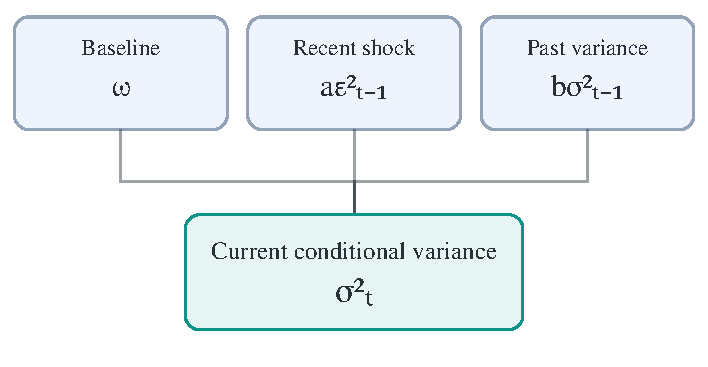
\includegraphics[width=\linewidth]{../reader_prototype/latex/figures/garch-mechanism.pdf}
\captionof{figure}{GARCH(1,1) 条件方差的组成}
\end{readerfigure}

GARCH 的基本思想是：当前波动率不仅取决于最近一次市场冲击，还受到此前波动率的影响。

\hypertarget{part-4-58-0007-proposition-unconditional-variance}{%
\paragraph{Proposition --- Unconditional Variance}\label{part-4-58-0007-proposition-unconditional-variance}}

假设存在具有有限二阶矩的平稳解，并满足：
\[a+b<1.\]

对条件方差方程两侧取期望：
\[\mathbb E[\sigma_t^2]
=
\omega
+a\mathbb E[\varepsilon_{t-1}^2]
+b\mathbb E[\sigma_{t-1}^2].\]

根据 Law of Total Expectation：
\[\begin{aligned}
\mathbb E[\varepsilon_{t-1}^2]
&=\mathbb E[
\mathbb E[\varepsilon_{t-1}^2
\mid\mathcal F_{t-2}]
]\\
&=\mathbb E[\sigma_{t-1}^2].
\end{aligned}\]

因此：
\[\mathbb E[\sigma_t^2]
=
\omega+(a+b)\mathbb E[\sigma_{t-1}^2].\]

由平稳性：
\[\mathbb E[\sigma_t^2]
=
\mathbb E[\sigma_{t-1}^2].\]

于是：
\[\boxed{
\mathbb E[\sigma_t^2]
=
\frac{\omega}{1-a-b}.
}\]

这同时也是上述模型中收益率的无条件方差。

\hypertarget{part-4-58-0007-volatility-persistence}{%
\paragraph{Volatility Persistence}\label{part-4-58-0007-volatility-persistence}}

设长期方差为：
\[\bar\sigma^2=\frac{\omega}{1-a-b}.\]

条件方差预测向长期方差回归的速度主要由 \(a+b\) 决定。

\begin{readerfigure}{0.72}
\figuretitle{GARCH --- Volatility Shock Persistence}
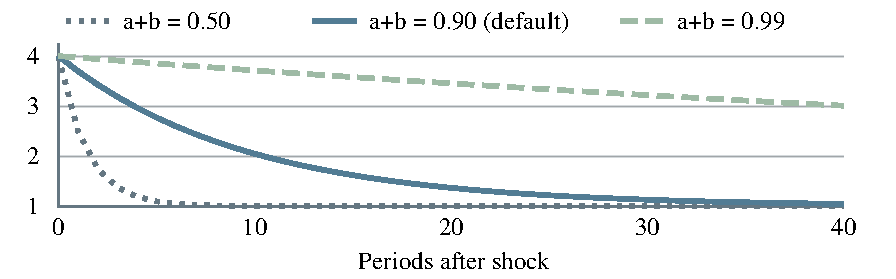
\includegraphics[width=\linewidth]{../reader_prototype/latex/figures/garch-persistence.pdf}

\smallskip
\begin{tabular}{@{}lrrr@{}}
\toprule
\(a+b\) & 0.50 & 0.90 & 0.99 \\
\midrule
Shock half-life（连续插值，Periods） & 1.00 & 6.58 & 68.97 \\
Remaining shock after 20 periods & 0.0\% & 12.2\% & 81.8\% \\
\bottomrule\end{tabular}
\captionof{figure}{归一化教学模型：长期方差为 1，初始超额方差为 3。曲线描述条件方差预测的恢复过程。}
\end{readerfigure}

这里有一个相当 Nontrivial 的观点：

\textbf{Conditional Variance 随时间变化，并不意味着 Unconditional Variance 随时间变化。}

GARCH 可以同时具有：

\begin{itemize}
\tightlist
\item
  Time-varying Conditional Variance；
\item
  Constant Unconditional Variance；
\item
  Weak Stationarity。
\end{itemize}

所以：
\[\boxed{
\text{Volatility Clustering}
\not\Rightarrow
\text{Non-stationarity}.
}\]

这一点非常容易混淆。

\hypertarget{part-4-58-0007-heavy-tailsux539aux5c3eux5206ux5e03}{%
\subsection{7. Heavy Tails（厚尾分布）}\label{part-4-58-0007-heavy-tailsux539aux5c3eux5206ux5e03}}

\hypertarget{part-4-58-0007-gaussian-assumption-ux7684ux5c40ux9650}{%
\subsubsection{7.1 Gaussian Assumption 的局限}\label{part-4-58-0007-gaussian-assumption-ux7684ux5c40ux9650}}

我们此前大量使用 Normal Distribution，因为它具有非常好的数学性质。

但是，现实金融收益率经常表现出比正态分布更厚的尾部，即极端观测值出现的概率比 Gaussian Model 所预期的更高。

\begin{readerfigure}{0.46}
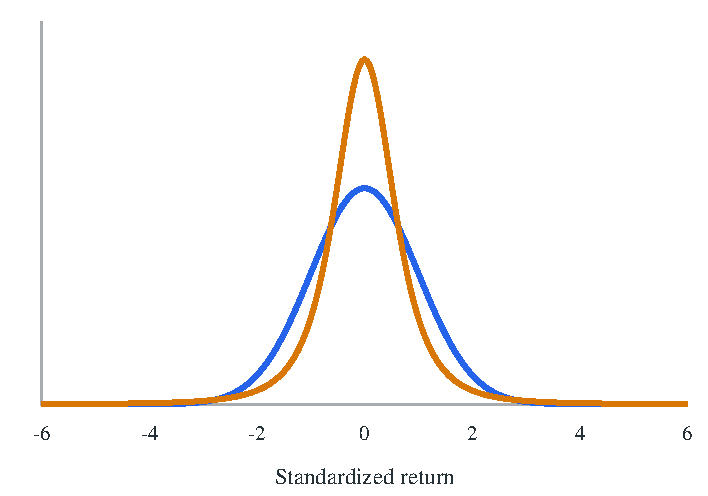
\includegraphics[width=\linewidth]{../reader_prototype/latex/figures/densities.pdf}
\par \legendmark{ResearchBlue}\,Standard Normal\enspace \legenddash{ResearchSlate}\,Standardized Student's t (ν=3)
\captionof{figure}{两种分布均具有零均值和单位方差，但尾部概率存在显著差异。}
\end{readerfigure}

例如，我们比较 Standard Normal Distribution 与标准化为单位方差的 Student's t Distribution（自由度为 3）。

\begin{readertable}
\begin{longtable}[]{@{}
  >{\raggedright\arraybackslash}p{(\columnwidth - 4\tabcolsep) * \real{0.33}}
  >{\raggedleft\arraybackslash}p{(\columnwidth - 4\tabcolsep) * \real{0.27}}
  >{\raggedleft\arraybackslash}p{(\columnwidth - 4\tabcolsep) * \real{0.36}}@{}}
\toprule
Extreme Event & Normal & Standardized \(t_3\) \\
\midrule
\endhead
超过 3 个标准差 & 0.270\% & 1.385\% \\
超过 5 个标准差 & 0.0000573\% & 0.324\% \\
\bottomrule
\end{longtable}
\end{readertable}

以上均为双侧理论尾部概率。

\begin{readerfigure}{0.72}
\figuretitle{Probability of a 5-standard-deviation event}
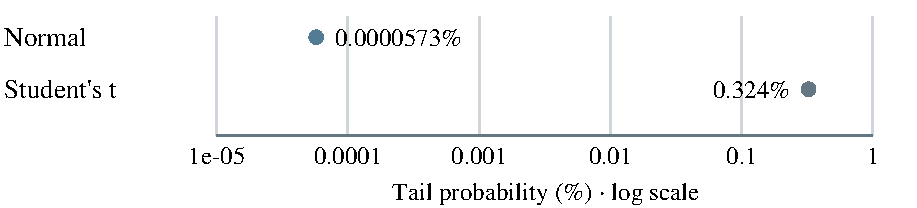
\includegraphics[width=\linewidth]{../reader_prototype/latex/figures/tail-probability.pdf}
\par\textbf{约 5,650 倍}
\captionof{figure}{即使均值和方差完全相同，极端事件概率也可能存在数量级差异。}
\end{readerfigure}

这也是为什么仅仅比较 Mean 和 Variance，可能不足以充分描述金融数据的风险特征。

\hypertarget{part-4-58-0007-moment-existenceux77e9ux7684ux5b58ux5728ux6027}{%
\subsubsection{7.2 Moment Existence（矩的存在性）}\label{part-4-58-0007-moment-existenceux77e9ux7684ux5b58ux5728ux6027}}

Student's t Distribution 具有一个值得关注的数学性质。

对于：
\[X\sim t_\nu,\]

其 \(p\) 阶绝对矩存在的条件为：
\[\boxed{
\mathbb E[|X|^p]<\infty
\iff p<\nu,
\qquad p>0.
}\]

\begin{readertable}
\begin{longtable}[]{@{}
  >{\raggedright\arraybackslash}p{(\columnwidth - 6\tabcolsep) * \real{0.33}}
  >{\raggedright\arraybackslash}p{(\columnwidth - 6\tabcolsep) * \real{0.16}}
  >{\raggedright\arraybackslash}p{(\columnwidth - 6\tabcolsep) * \real{0.20}}
  >{\raggedright\arraybackslash}p{(\columnwidth - 6\tabcolsep) * \real{0.27}}@{}}
\toprule
Degrees of Freedom & Mean & Variance & Fourth Moment \\
\midrule
\endhead
\(\nu=1\) & 不存在 & 不存在 & 不存在 \\
\(\nu=2\) & 存在 & 不存在 & 不存在 \\
\(\nu=3\) & 存在 & 存在 & 不存在 \\
\(\nu=5\) & 存在 & 存在 & 存在 \\
\bottomrule
\end{longtable}
\end{readertable}

其中：
\[t_1=\text{Cauchy Distribution}.\]

也就是此前 Probability 中学习过的 Cauchy Distribution。

\hypertarget{part-4-58-0007-proof-sketch}{%
\paragraph{Proof Sketch}\label{part-4-58-0007-proof-sketch}}

Student's t Distribution 的概率密度为：
\[f_\nu(x)
=
\frac{
\Gamma((\nu+1)/2)
}{
\sqrt{\nu\pi}\Gamma(\nu/2)
}
\left(1+\frac{x^2}{\nu}\right)^{-(\nu+1)/2}.\]

当 \(|x|\to\infty\) 时：
\[f_\nu(x)\asymp |x|^{-(\nu+1)}.\]

因此，绝对矩积分的尾部行为为：
\[\int^\infty x^pf_\nu(x)\,\mathrm dx
\asymp
\int^\infty x^{p-\nu-1}\,\mathrm dx.\]

根据 Improper Integral 的收敛条件：
\[p-\nu-1<-1,\]

即：
\[\boxed{p<\nu.}\]

\hypertarget{part-4-58-0007-heavy-tails-ux5bf9ux7edfux8ba1ux5b66ux4e60ux7684ux5f71ux54cd}{%
\subsubsection{7.3 Heavy Tails 对统计学习的影响}\label{part-4-58-0007-heavy-tails-ux5bf9ux7edfux8ba1ux5b66ux4e60ux7684ux5f71ux54cd}}

现在回顾 Part II 中使用过的几个数学工具。

\begin{readertable}
\begin{longtable}[]{@{}
  >{\raggedright\arraybackslash}p{(\columnwidth - 4\tabcolsep) * \real{0.32}}
  >{\raggedright\arraybackslash}p{(\columnwidth - 4\tabcolsep) * \real{0.29}}
  >{\raggedright\arraybackslash}p{(\columnwidth - 4\tabcolsep) * \real{0.35}}@{}}
\toprule
Statistical Tool & Relevant Assumption & Potential Problem \\
\midrule
\endhead
Chebyshev Inequality & Finite Variance & 方差可能不存在 \\
Classical IID CLT & Finite Variance & 极限分布可能不是正态 \\
Hoeffding Inequality & Bounded Variables & 收益率或损失函数可能无界 \\
Sample Variance Inference & 通常涉及高阶矩条件 & 方差估计本身可能非常不稳定 \\
Standard Bootstrap & 依赖统计量及分布条件 & 厚尾可能影响重采样推断 \\
\bottomrule
\end{longtable}
\end{readertable}

尤其需要注意一种情况：

假设预测误差具有有限二阶矩，却没有有限四阶矩。

那么对于 Squared Loss：
\[L=\varepsilon^2,\]

我们可能有：
\[\mathbb E[L]=\mathbb E[\varepsilon^2]<\infty,\]

但：
\[\operatorname{Var}(L)
=
\mathbb E[\varepsilon^4]
-\mathbb E[\varepsilon^2]^2
=\infty.\]

也就是说，\textbf{Population MSE 可以存在，但经验 MSE 的方差可能不存在。}

这使得两个模型之间微小的 MSE Improvement 更难被可靠识别。

对于 Financial RSI，Agent 可能不断根据高度不稳定的 Evaluation Score 修改自身，并将偶然出现的极端结果误认为真实研究规律。

当然，金融数据具有厚尾，并不意味着它一定没有有限方差。上述结论取决于具体 DGP 与所使用的损失函数。

\hypertarget{part-4-58-0007-temporal-dependence-and-effective-sample-size}{%
\subsection{8. Temporal Dependence and Effective Sample Size}\label{part-4-58-0007-temporal-dependence-and-effective-sample-size}}

这是本阶段与 Part II 联系最紧密的数学内容之一。

\hypertarget{part-4-58-0007-ux4e2aux89c2ux6d4bux503cux4e0dux4e00ux5b9aux5bf9ux5e94-1000-ux4efdux72ecux7acbux4fe1ux606f}{%
\subsubsection{8.1 1,000 个观测值不一定对应 1,000 份独立信息}\label{part-4-58-0007-ux4e2aux89c2ux6d4bux503cux4e0dux4e00ux5b9aux5bf9ux5e94-1000-ux4efdux72ecux7acbux4fe1ux606f}}

对于 IID Random Variables：
\[\operatorname{Var}(\bar X_n)
=
\frac{\sigma^2}{n}.\]

然而，当观测值存在时间依赖时，这个关系不再普遍成立。

设 \(\{X_t\}\) 为弱平稳随机过程，并定义：
\[\gamma_h
=
\operatorname{Cov}(X_t,X_{t+h}),\]

\[\rho_h=\frac{\gamma_h}{\gamma_0}.\]

那么：
\[\boxed{
\operatorname{Var}(\bar X_n)
=
\frac{\gamma_0}{n}
\left[
1+
2\sum_{h=1}^{n-1}
\left(1-\frac hn\right)\rho_h
\right].
}\]

这实际上就是我们在 II-F 中使用过的时间序列样本均值方差公式。

\hypertarget{part-4-58-0007-proof}{%
\paragraph{Proof}\label{part-4-58-0007-proof}}

\[\begin{aligned}
\operatorname{Var}(\bar X_n)
&=
\operatorname{Var}
\left(
\frac1n\sum_{t=1}^nX_t
\right)\\
&=\frac1{n^2}
\sum_{i=1}^n
\sum_{j=1}^n
\operatorname{Cov}(X_i,X_j).
\end{aligned}\]

利用弱平稳性，将相同 Lag 的协方差项合并：
\[\operatorname{Var}(\bar X_n)
=
\frac1{n^2}
\left[
n\gamma_0
+2\sum_{h=1}^{n-1}(n-h)\gamma_h
\right].\]

提取公因子即可得到上述结果。

\hypertarget{part-4-58-0007-effective-sample-size}{%
\subsubsection{8.2 Effective Sample Size}\label{part-4-58-0007-effective-sample-size}}

为了刻画时间依赖对样本均值估计的影响，我们定义：
\[\boxed{
n_{\mathrm{eff}}
=
\frac{n}{
1+
2\sum_{h=1}^{n-1}
(1-h/n)\rho_h
}.
}\]

在分母为正的条件下，有：
\[\operatorname{Var}(\bar X_n)
=
\frac{\gamma_0}{n_{\mathrm{eff}}}.\]

这里的 \(n_{\mathrm{eff}}\) 称为 Effective Sample Size（有效样本量）。

其含义是：对于样本均值估计，当前相关序列的方差，相当于多少个具有相同边际方差的独立观测值所产生的方差。

需要注意，Effective Sample Size 是针对具体统计量定义的，并不是一份数据集唯一且固定的属性。

\hypertarget{part-4-58-0007-ar1-example}{%
\subsubsection{8.3 AR(1) Example}\label{part-4-58-0007-ar1-example}}

沿用 §5.2 中的模型：
\[X_t=\phi X_{t-1}+\varepsilon_t,\]

其中：
\[|\phi|<1.\]

我们已经得到：
\[\rho_h=\phi^{|h|}.\]

当 \(n\) 足够大、\(\phi\) 固定时：
\[\begin{aligned}
1+2\sum_{h=1}^{\infty}\phi^h
&=1+\frac{2\phi}{1-\phi}\\
&=\frac{1+\phi}{1-\phi}.
\end{aligned}\]

因此：
\[\boxed{
n_{\mathrm{eff}}
\approx
n\frac{1-\phi}{1+\phi}.
}\]

\textbf{Effective Sample Size Explorer}

Nominal sample size \(n\)\\
\textbf{1,000}

1000（范围 100--5000）

Autocorrelation parameter \(\phi\)\\
\textbf{0.80}

0.8（范围 0--0.95）

Nominal sample size

\begin{verbatim}
  **1,000**
\end{verbatim}

Effective sample size

\begin{verbatim}
  **112**
\end{verbatim}

Effective information ratio

\textbf{11.2\%}

Standard error multiplier

\textbf{2.99×}

基于平稳 AR(1) 的有限样本方差公式计算，而非真实金融市场的估计结果。

对于 \(n=1000\)，可以得到如下渐近近似结果。

\begin{readertable}
\begin{longtable}[]{@{}
  >{\raggedleft\arraybackslash}p{(\columnwidth - 4\tabcolsep) * \real{0.15}}
  >{\raggedleft\arraybackslash}p{(\columnwidth - 4\tabcolsep) * \real{0.39}}
  >{\raggedleft\arraybackslash}p{(\columnwidth - 4\tabcolsep) * \real{0.42}}@{}}
\toprule
\(\phi\) & Nominal Sample Size & Effective Sample Size \\
\midrule
\endhead
0.0 & 1,000 & 1,000 \\
0.2 & 1,000 & 667 \\
0.5 & 1,000 & 333 \\
0.8 & 1,000 & 111 \\
0.9 & 1,000 & 53 \\
0.95 & 1,000 & 26 \\
\bottomrule
\end{longtable}
\end{readertable}

因此，较强的正向时间依赖可能显著降低有效样本信息量。负自相关则可能使针对样本均值定义的有效样本量超过原始样本量。

\hypertarget{part-4-58-0007-ux4e00ux4e2aux4e0e-rsi-ux76f4ux63a5ux76f8ux5173ux7684-nontrivial-example}{%
\subsubsection{8.4 一个与 RSI 直接相关的 Nontrivial Example}\label{part-4-58-0007-ux4e00ux4e2aux4e0e-rsi-ux76f4ux63a5ux76f8ux5173ux7684-nontrivial-example}}

假设我们的金融预测任务使用未来五期的累计 Log Return 作为 Label。

定义：
\[Y_t=\sum_{j=1}^{5}r_{t+j}^{\log}.\]

为了简化分析，假设单期 Log Return 为 IID：
\[r_t^{\log}\sim(0,\sigma^2).\]

即使原始收益率完全独立，相邻 Label 仍然存在重叠。

\textbf{Overlapping Return Labels}

\bookgraphic{0.693}{part-4-58-0007-008-01}{相邻五期累计收益率共享四个原始收益率观测值。}

由于：
\[Y_t=r_{t+1}^{\log}+\cdots+r_{t+5}^{\log},\]

\[Y_{t+1}=r_{t+2}^{\log}+\cdots+r_{t+6}^{\log},\]

因此：
\[\operatorname{Cov}(Y_t,Y_{t+1})
=
4\sigma^2.\]

又因为：
\[\operatorname{Var}(Y_t)=5\sigma^2,\]

所以：
\[\boxed{
\operatorname{Corr}(Y_t,Y_{t+1})
=
\frac45=0.8.
}\]

更加一般地，对于长度为 \(H\) 的累计 Log Return：
\[Y_t=\sum_{j=1}^{H}r_{t+j}^{\log},\]

在上述 IID 假设下：
\[\boxed{
\rho_h=
\begin{cases}
1-\dfrac{|h|}{H},&|h|<H,\\
0,&|h|\geq H.
\end{cases}
}\]

因此，当 \(n\) 足够大时：
\[\begin{aligned}
n_{\mathrm{eff}}
&\approx
\frac{n}{
1+2\sum_{h=1}^{H-1}(1-h/H)
}\\
&=\frac{n}{H}.
\end{aligned}\]

也就是说：
\[\boxed{
n_{\mathrm{eff}}\approx\frac nH.
}\]

假如我们拥有 1,000 个相互重叠的 20 日收益率标签，其均值估计的有效样本量可能仅相当于约 50 个独立标签。

这也进一步解释了 II-F 中为什么需要 Purging、Label Availability Check 和 dependence-aware Statistical Inference。 注意：这个有效样本量公式针对上述 IID 增量模型中的标签均值，不能直接套用到所有模型损失或策略收益上。

\hypertarget{part-4-58-0007-ux4e3aux4ec0ux4e48ux91d1ux878dux73afux5883ux7279ux522bux5bb9ux6613ux4ea7ux751f-rsi-overfitting}{%
\subsection{9. 为什么金融环境特别容易产生 RSI Overfitting？}\label{part-4-58-0007-ux4e3aux4ec0ux4e48ux91d1ux878dux73afux5883ux7279ux522bux5bb9ux6613ux4ea7ux751f-rsi-overfitting}}

现在可以将本阶段的内容与 Part II 和 Part III 连接起来。

\begin{readertable}
\begin{longtable}[]{@{}
  >{\raggedright\arraybackslash}p{(\columnwidth - 4\tabcolsep) * \real{0.29}}
  >{\raggedright\arraybackslash}p{(\columnwidth - 4\tabcolsep) * \real{0.31}}
  >{\raggedright\arraybackslash}p{(\columnwidth - 4\tabcolsep) * \real{0.37}}@{}}
\toprule
Financial Property & Statistical Consequence & RSI Consequence \\
\midrule
\endhead
Weak Predictability & 真实模型差异可能很小 & 容易选择噪声驱动的修改 \\
Temporal Dependence & 有效样本信息可能减少 & 评估可靠性下降 \\
Heavy Tails & 极端观测可能主导指标 & Agent 可能过度优化偶然事件 \\
Volatility Clustering & 条件方差随时间变化 & 不同市场窗口的评分稳定性不同 \\
Non-stationarity & 历史规律可能失效 & 后期版本可能过度适应旧环境 \\
Single Historical Path & 缺少独立市场历史 & 反复回测可能累积选择偏差 \\
\bottomrule
\end{longtable}
\end{readertable}

\textbf{Coding Tasks}

部分正确性可以确定性验证

反馈相对明确

\textbf{Financial Tasks}

真实性能难以直接观测

评估反馈可能包含大量噪声

↓

\textbf{Same RSI Architecture} \(A_0\rightarrow A_1\rightarrow\cdots\rightarrow A_K\)

↓

\bookgraphic{0.591}{part-4-58-0007-009-01}{}

IS Performance

Potential OOS trajectory in a reliable evaluation environment

Potential OOS trajectory in a low-SNR financial environment

研究假设示意，并非真实实验结果。编程任务同样可能发生严重过拟合。

这里最重要的认识是：

\textbf{金融环境未必削弱 Agent 的 Optimization Capability，却可能显著削弱 Evaluator 区分真实改进与虚假改进的能力。}

Agent 仍然可以变得越来越擅长搜索，但它所搜索到的高分候选未必代表真正的能力提升。

\hypertarget{part-4-58-0007-research-practice-initial-financial-data-audit}{%
\subsection{10. Research Practice --- Initial Financial Data Audit}\label{part-4-58-0007-research-practice-initial-financial-data-audit}}

假设未来课题组向我们提供了一份金融数据，我们不应该立即开始运行 RSI。

第一步应当对 DGP 的统计特征进行初步分析。

\hypertarget{part-4-58-0007-diagnostic-framework}{%
\subsubsection{10.1 Diagnostic Framework}\label{part-4-58-0007-diagnostic-framework}}

\begin{readertable}
\begin{longtable}[]{@{}
  >{\raggedright\arraybackslash}p{(\columnwidth - 4\tabcolsep) * \real{0.32}}
  >{\raggedright\arraybackslash}p{(\columnwidth - 4\tabcolsep) * \real{0.37}}
  >{\raggedright\arraybackslash}p{(\columnwidth - 4\tabcolsep) * \real{0.27}}@{}}
\toprule
Diagnostic & Method & Research Purpose \\
\midrule
\endhead
Return Transformation & Simple / Log Return & 统一统计对象 \\
Distribution Analysis & Histogram、Q-Q Plot & 检查厚尾及偏度 \\
Temporal Dependence & ACF of Returns & 检查线性依赖 \\
Volatility Dependence & ACF of Absolute / Squared Returns & 检查波动率聚集 \\
Rolling Statistics & Rolling Mean / Variance & 调查潜在结构变化 \\
Information Availability & Timestamp Audit & 排除 Look-Ahead Bias \\
Sample Size Analysis & Effective Sample Size & 判断评估不确定性 \\
\bottomrule
\end{longtable}
\end{readertable}

\hypertarget{part-4-58-0007-python-implementation}{%
\subsubsection{10.2 Python Implementation}\label{part-4-58-0007-python-implementation}}

一个基本的 Exploratory Data Analysis 可以写成：

\begin{verbatim}
import numpy as np
import pandas as pd
import matplotlib.pyplot as plt

from statsmodels.graphics.tsaplots import plot_acf
from scipy.stats import probplot

# Assume df contains chronologically indexed prices.
df = df.sort_index()

# Log returns
r = np.log(df["close"]).diff().dropna()

fig, axes = plt.subplots(2, 3, figsize=(14, 7))

# 1. Distribution
axes[0, 0].hist(r, bins=60, density=True)
axes[0, 0].set_title("Return Distribution")

# 2. Normal Q-Q plot
probplot(r, dist="norm", plot=axes[0, 1])
axes[0, 1].set_title("Normal Q-Q Plot")

# 3. Rolling volatility
r.rolling(60).std().plot(ax=axes[0, 2])
axes[0, 2].set_title("Rolling Volatility")

# 4. Return autocorrelation
plot_acf(r, lags=30, ax=axes[1, 0])
axes[1, 0].set_title("ACF of Returns")

# 5. Absolute return autocorrelation
plot_acf(r.abs(), lags=30, ax=axes[1, 1])
axes[1, 1].set_title("ACF of Absolute Returns")

# 6. Squared return autocorrelation
plot_acf(r**2, lags=30, ax=axes[1, 2])
axes[1, 2].set_title("ACF of Squared Returns")

plt.tight_layout()
plt.show()
\end{verbatim}

这段代码尚未在课题组数据上实际运行，假设价格为正且数据量足够。实际使用时需要处理复权价格、缺失值、交易日对齐及 ACF 置信区间的适用条件。

尤其需要注意，如果这些探索性分析将用于设计 RSI 策略，那么应该只在 Development Dataset 上进行，而不是提前分析封闭的 Final Test Dataset。

否则，人类研究人员也可能发生我们在 II-F 中讨论过的 Researcher-level Overfitting。

\hypertarget{part-4-58-0007-literature-index}{%
\subsection{11. Literature Index}\label{part-4-58-0007-literature-index}}

本阶段不需要立刻学习完整的 Financial Econometrics 教材，优先掌握以下经典文献即可。

\textbf{P0 --- Empirical Properties of Asset Returns: Stylized Facts and Statistical Issues}

Rama Cont · 2001 · Quantitative Finance, 1(2), 223--236 · 同行评审

本阶段最重要的参考文献。重点理解收益率分布、非线性依赖、Volatility Clustering 和金融统计估计困难。

\href{https://doi.org/10.1080/713665670}{DOI: 10.1080/713665670}

\textbf{P1 --- Generalized Autoregressive Conditional Heteroskedasticity}

Tim Bollerslev · 1986 · Journal of Econometrics, 31(3), 307--327 · 同行评审

GARCH 的经典原始论文。现阶段理解 Model Specification 与 Stationarity 即可，不需要深入 Maximum Likelihood Estimation。

\href{https://doi.org/10.1016/0304-4076(86)90063-1}{DOI: 10.1016/0304-4076(86)90063-1}

本次补发没有重新进行文献检索。这里保留上述两篇经典文献作为主要阅读入口。

\hypertarget{part-4-58-0007-iv-a-conclusion-index}{%
\subsection{12. IV-A --- Conclusion Index}\label{part-4-58-0007-iv-a-conclusion-index}}

\hypertarget{part-4-58-0007-core-conclusions}{%
\subsubsection{12.1 Core Conclusions}\label{part-4-58-0007-core-conclusions}}

\begin{readertable}
\begin{longtable}[]{@{}
  >{\raggedright\arraybackslash}p{(\columnwidth - 4\tabcolsep) * \real{0.13}}
  >{\raggedright\arraybackslash}p{(\columnwidth - 4\tabcolsep) * \real{0.70}}
  >{\raggedright\arraybackslash}p{(\columnwidth - 4\tabcolsep) * \real{0.13}}@{}}
\toprule
ID & Key Conclusion & Index \\
\midrule
\endhead
A1 & Simple Return 通过乘法累积，Log Return 通过加法累积 & §1 \\
A2 & 一条历史序列只是随机过程的一条 Sample Path & §2.1 \\
A3 & Filtration 定义金融预测中的合法信息集合 & §2.2 \\
A4 & Conditional Mean 与 Conditional Variance 是不同预测目标 & §3 \\
A5 & Stationarity 不等于 Independence & §4 \\
A6 & Random Walk 的价格非平稳，但其增量可以平稳 & §4.3 \\
A7 & ACF 衡量时间序列的线性依赖 & §5 \\
A8 & 零自相关不意味着不存在非线性时间依赖 & §6.3 \\
A9 & Volatility Clustering 不必然意味着 Non-stationarity & §6.4 \\
A10 & Heavy Tails 可能限制传统统计推断方法的适用性 & §7 \\
A11 & Temporal Dependence 会改变有效样本信息量 & §8 \\
A12 & 金融数据特性可能降低 RSI Evaluator 的可靠性 & §9 \\
\bottomrule
\end{longtable}
\end{readertable}

\hypertarget{part-4-58-0007-core-formula-sheet}{%
\subsubsection{12.2 Core Formula Sheet}\label{part-4-58-0007-core-formula-sheet}}

\hypertarget{part-4-58-0007-result-1-return-transformation}{%
\paragraph{Result 1 --- Return Transformation}\label{part-4-58-0007-result-1-return-transformation}}

\[r_t=\frac{P_t-P_{t-1}}{P_{t-1}},\]

\[r_t^{\log}=\log(1+r_t).\]

\hypertarget{part-4-58-0007-result-2-financial-dgp}{%
\paragraph{Result 2 --- Financial DGP}\label{part-4-58-0007-result-2-financial-dgp}}

\[r_{t+1}
=
\mu_t+\sigma_tZ_{t+1}.\]

\hypertarget{part-4-58-0007-result-3-ar1}{%
\paragraph{Result 3 --- AR(1)}\label{part-4-58-0007-result-3-ar1}}

\[X_t=\phi X_{t-1}+\varepsilon_t.\]

在相应平稳条件下：
\[\operatorname{Var}(X_t)
=
\frac{\sigma_\varepsilon^2}{1-\phi^2},\]

\[\rho_h=\phi^{|h|}.\]

\hypertarget{part-4-58-0007-result-4-garch11}{%
\paragraph{Result 4 --- GARCH(1,1)}\label{part-4-58-0007-result-4-garch11}}

\[\sigma_t^2
=
\omega+a\varepsilon_{t-1}^2+b\sigma_{t-1}^2.\]

在有限二阶矩平稳条件下：
\[\boxed{
\mathbb E[\sigma_t^2]
=
\frac{\omega}{1-a-b}.
}\]

\hypertarget{part-4-58-0007-result-5-moment-existence-of-students-t}{%
\paragraph{Result 5 --- Moment Existence of Student's t}\label{part-4-58-0007-result-5-moment-existence-of-students-t}}

\[X\sim t_\nu
\quad\Longrightarrow\quad
\mathbb E[|X|^p]<\infty
\iff p<\nu.\]

\hypertarget{part-4-58-0007-result-6-effective-sample-size}{%
\paragraph{Result 6 --- Effective Sample Size}\label{part-4-58-0007-result-6-effective-sample-size}}

\[n_{\mathrm{eff}}
=
\frac{n}{
1+2\sum_{h=1}^{n-1}(1-h/n)\rho_h
}.\]

对于平稳 AR(1)：
\[\boxed{
n_{\mathrm{eff}}
\approx
n\frac{1-\phi}{1+\phi}.
}\]

\hypertarget{part-4-58-0007-result-7-overlapping-return-labels}{%
\paragraph{Result 7 --- Overlapping Return Labels}\label{part-4-58-0007-result-7-overlapping-return-labels}}

对于 IID 单期收益率构成的 \(H\) 期累计收益率标签：
\[\rho_h=
\begin{cases}
1-\dfrac{|h|}{H},&|h|<H,\\
0,&|h|\geq H.
\end{cases}\]

当 \(n\) 足够大时，针对标签均值：
\[\boxed{
n_{\mathrm{eff}}\approx\frac nH.
}\]

\hypertarget{part-4-58-0007-proof-index}{%
\subsubsection{12.3 Proof Index}\label{part-4-58-0007-proof-index}}

如果第二轮学习时希望重点复习数学推导，可以直接索引下表。

\begin{readertable}
\begin{longtable}[]{@{}
  >{\raggedright\arraybackslash}p{(\columnwidth - 4\tabcolsep) * \real{0.14}}
  >{\raggedright\arraybackslash}p{(\columnwidth - 4\tabcolsep) * \real{0.61}}
  >{\raggedright\arraybackslash}p{(\columnwidth - 4\tabcolsep) * \real{0.20}}@{}}
\toprule
Proof & Mathematical Result & Location \\
\midrule
\endhead
P1 & Log Return 的 Time Additivity & §1.3 \\
P2 & Random Walk 的 Non-stationarity & §4.3 \\
P3 & 零自相关但平方序列相关的反例 & §6.3 \\
P4 & GARCH 的 Unconditional Variance & §6.4 \\
P5 & Student's t 的矩存在条件 & §7.2 \\
P6 & 相关序列的样本均值方差 & §8.1 \\
P7 & AR(1) 的 Effective Sample Size & §8.3 \\
P8 & Overlapping Labels 的相关性及有效样本量 & §8.4 \\
\bottomrule
\end{longtable}
\end{readertable}

\hypertarget{part-4-58-0007-research-takeaway}{%
\subsection{13. Research Takeaway}\label{part-4-58-0007-research-takeaway}}

将整个 IV-A 压缩为一个核心观点：

\textbf{金融 RSI 面临的困难，不仅是需要从高噪声数据中寻找规律，还需要在同一批有限、相关且可能非平稳的数据中，反复判断哪些研究修改是真正有效的。}

我们可以用如下概念关系将其与之前的内容连接起来。

\textbf{Agent Capability}

Part III

Search、Memory、RSI

\textbf{Evaluator Reliability}

Part II + Part IV

Statistics、Financial DGP

↓

\textbf{Optimization--Evaluation Mismatch}

优化能力提高的速度可能超过评价机制可靠性提高的速度

↓

\textbf{Potential Generalization Decay} \(S_k^{\mathrm{IS}}\uparrow,\qquad S_k^{\mathrm{OOS}}\downarrow\)

这仍然是一种需要受控实验验证的研究假设，而不是金融 RSI 必然遵守的定律。

\hypertarget{part-4-58-0007-next-iv-b-low-signal-to-noise-ratio-predictability}{%
\subsection{Next --- IV-B: Low Signal-to-Noise Ratio \& Predictability}\label{part-4-58-0007-next-iv-b-low-signal-to-noise-ratio-predictability}}

IV-A --- Financial Time Series \& DGP

IV-B --- Low Signal-to-Noise Ratio \& Predictability

IV-C --- Financial Factors \& ML Models

IV-D --- Returns, Sharpe Ratio \& Evaluation

IV-E --- Backtest Overfitting, PBO \& DSR

IV-F --- Market Regime \& Robustness

下一阶段是 Part IV 中理论优先级最高的一节。

\begin{readertable}
\begin{longtable}[]{@{}
  >{\raggedright\arraybackslash}p{(\columnwidth - 2\tabcolsep) * \real{0.41}}
  >{\raggedright\arraybackslash}p{(\columnwidth - 2\tabcolsep) * \real{0.55}}@{}}
\toprule
Topic & Core Question \\
\midrule
\endhead
Signal-to-Noise Ratio & 如何定量描述金融预测的困难？ \\
Law of Total Variance & 如何分解可预测与不可预测成分？ \\
Irreducible Error & 模型性能的理论上限在哪里？ \\
Bayes Optimal Predictor & 最好的预测器在数学上是什么？ \\
Population \(R^2\) & 低信噪比如何限制预测能力？ \\
Efficient Market Hypothesis & 为什么金融规律可能难以持续利用？ \\
Spurious Correlation & 为什么无效金融特征也可能获得极高得分？ \\
Noise-driven Optimization & RSI 如何逐步将噪声误认为真实改进？ \\
\bottomrule
\end{longtable}
\end{readertable}

特别是，我们将利用你已经掌握的 Conditional Expectation 与 Law of Total Variance 推导：
\[\boxed{
R_{\mathrm{optimal}}^2
=
\frac{\mathrm{SNR}}{1+\mathrm{SNR}}
}\]

\textbf{Signal-to-Noise Ratio vs. Optimal Predictability}

\bookgraphic{0.473}{part-4-58-0007-013-01}{理论关系预览：在平方损失、有限二阶矩及特定 SNR 定义下成立。}

这个等式将金融数据的信噪比与理论最优预测能力直接联系起来。

而 IV-B 真正值得研究的地方就在于：\textbf{即使 Agent 具有无限强大的优化能力，它也无法突破给定信息集合所决定的理论预测上限。}
